\documentclass[twoside,a4paper,11pt]{memoir}
\usepackage{times}
\usepackage{pslatex}
\usepackage{url}
\usepackage{mscthesis}
\let\newfloat\undefined \usepackage{algorithmic} 
\usepackage{algorithm}
\usepackage{graphicx}
\usepackage{color}
\usepackage{hyperref}
\usepackage{adjustbox}
\usepackage{xspace}
\usepackage{enumitem}

\newcommand{\etal}{\emph{et al.}\xspace}
\newcommand\todo[1]{\textcolor{red}{TODO: #1}}

\def\chapterautorefname{Chapter} 
\def\sectionautorefname{Section} 
\def\subsectionautorefname{Section} 

\title{DDU}
\subtitle{Master's Thesis}

\author{Aaron Ang}
\authoremail{\url{a.w.z.ang@student.tudelft.nl}}
\birthplace{Amstelveen, The Netherlands}
\studentid{4139194}

\company{

\includegraphics[height=1.3cm]{figures/parc_logo.png}\\
PARC, a Xerox company\\
3333 Coyote Hill Road\\
Palo Alto, CA 94304\\
\url{www.parc.com}
}

\chair{Prof. Dr. A. van Deursen, Faculty EEMCS, TU Delft}
\supervisor{Prof. Dr. A. van Deursen, Faculty EEMCS, TU Delft}
\externalsupervisor{Prof. Dr. R. Maranhao, University of Lisbon}

\setcounter{tocdepth}{1}
\setsecnumdepth{subsection}
\maxsecnumdepth{subsection}

\begin{document}

\frontmatter
\thispagestyle{empty}
\maketitle
\makeformaltitlepages{ABSTRACT}

\chapter{Preface}
\label{ch:preface}

This is where you thank people for helping you etc.

\vskip1cm
\begin{flushright}
\theauthor\\
Delft, The Netherlands \\
\today\\
\end{flushright}

\cleardoublepage\tableofcontents
\cleardoublepage\listoffigures
\cleardoublepage\mainmatter

\chapter{Introduction}
\label{ch:introduction}
Software systems are complex and error-prone, likely to expose failures to the end user.
When a failure occurs, the developer has to debug the system to eliminate the failure.
This debugging process can be described in three phases \cite{parnin2011automated}.
In the first phase, the developer has to pinpoint the fault, also known as the root cause, in code that causes the failure.
In the second phase, the developer has to develop an understanding of the root cause and its context.
Finally, in the third phase, the developer has to implement a patch that corrects the behavior of the system.
This process is time-consuming and can account for 30\% to 90\% of the software development cycle \cite{robbins2003debugging, beizer2003software, britton2013reversible}.

Traditionally, developers use four different approaches to debug a software system, namely program logging, assertions, breakpoints and profiling \cite{wong2016survey}.
Program logging is the act of inserting \emph{print} statements in the code to observe program state information during execution.
Assertions are constraints that can be added to a program that have to evaluate to true during execution time.
Breakpoints allow the developer to pause the software system during execution, and observe and modify variable values.
Profiling is used to perform runtime analysis and collect metrics on, for example, execution speed and memory usage.
These techniques provide an intuitive approach to localize the root cause of a failure, but, as one might expect, are less effective in the massive size and scale of software systems today.

Therefore, in the last decades a lot of research has been performed on improving and developing \emph{advanced} fault localization techniques \cite{wong2016survey} such that they are applicable to the software systems of today.
Specifically, a prominent fault localization technique is spectrum-based fault localization (SBFL).
SBFL techniques pinpoint faults in code based on execution information of a program, also known as a program spectrum \cite{reps1997use}.
It does this by outputting a list of suspicious components, for example statements or methods, ranked by their suspiciousness.
Intuitively, if a statement is executed primarily during failed executions, then this statement might be assigned a higher suspiciousness score.
Similarly, if a statement is executed primarily during successful executions, then this statement might be assigned a lower suspiciousness score.

While SBFL techniques are promising for debugging purposes, these techniques are dependent on the quality of a test suite.
Currently, test suites are optimized with respect to adequacy measurements that focus on error detection, e.g. branch coverage, line coverage.
However, Perez \etal~\cite{DBLP:conf/icse/PerezAD17} show evidence that optimizing a test suite with respect to DDU --- a metric to quantify the test suite's diagnosability --- improves the diagnostic performance of SBFL by 34\% compared to a test suite optimized with respect to branch coverage.
The goal of DDU is to capture diagnosability and to serve as a complementary metric to code coverage for developers to use to improve the test suite's diagnosability.

\section{Problem Definition}
\label{sec:problem_definition}
Currently, when the DDU is computed for a given test suite, its value is in the domain $[ 0, 1 ]$, where $0$ suggests that the test suite's diagnosability is low, and $1$ suggests that the test suite's diagnosability is high.
The problem with this value is that the developer does not know how to extend or update the test suite given a DDU value.
For example, when the test suite's DDU is equal to $0.1$, the developer does not know how to write tests that improve the DDU.
In other words, time spent on software debugging cannot be reduced using DDU because its practical implications are unclear to the developer.

\section{Goal}
Although DDU is currently not usable in practice, Perez \etal \cite{DBLP:conf/icse/PerezAD17} have shown that optimizing a test suite with respect to DDU can yield a 34\% gain in diagnostic performance using SBFL.
In addition, having a test suite with a high diagnosability could possibly reduce the time spent debugging because the fault is easier to find manually.
Therefore, the goal of this thesis is to find ways to make DDU usable in practice.
In other words, we explore possibilities to convey DDU to the developer such that the developer knows what kind of tests to write to improve the system's diagnosability.
To be able to


\section{Structure of Report}
The structure of this report is as follows.
\todo{Update once all chapters are done.}

\chapter{Background}
\label{ch:background}

In this chapter, we discuss topics that are relevant to understanding the following chapters.
First, we discuss spectrum-based reasoning, which is used in the experiments to compute the diagnostic performance.
Second, we discuss the metric used to evaluate the diagnostic performance of spectrum-based fault localization techniques.
Then, we explain the definition of diagnosability and diagnosability metrics.
Finally, we briefly discuss error detection.

\section{Spectrum-Based Reasoning (SBR)}
\todo{Describe how SR works and Barinel.}

Spectrum-based reasoning is a spectrum-based fault localization technique that leverages a Bayesian reasoning framework to diagnose fault candidates that could potentially be the root cause for a given software failure \cite{abreu2009spectrum}.
In SBR, we define a finite set $\mathcal{C} = \langle c_1, c_2, \ldots, c_M \rangle$ of $M$ system components, and the finite set $\mathcal{T} = \langle t_1, t_2, \ldots, t_N \rangle$ of $N$ system transactions, such as test executions.
The outcomes of all system transactions are defined as an error vector $e = \langle e_1, e_2, \ldots, e_N \rangle$, where $e_i = 1$ indicates that transaction $t_i$ has failed and $e_i = 0$ otherwise.
To keep track of which system components were executed during which system transactions, we construct a $N \times M$ activity matrix $\mathcal{A}$, where $\mathcal{A}_{ij} = 1$ indicates that component $c_j$ was hit during transaction $t_i$.
The pair $(\mathcal{A}, e)$ is also known as a program spectrum, which was first coined by Reps \etal \cite{reps1997use}.

SBR distinguishes itself from SBFL techniques by leveraging a reasoning framework.
More specifically, the diagnostic report is generated by reasoning about the program spectrum instead of using a so-called similarity coefficient.

\section{Evaluation of Diagnosis}
\todo{Describe wasted effort}

\section{Diagnosability}
\todo{Explain concept and definition of diagnosability: the property of faults to be easily and precisely located}

\subsection{Diagnosability Metric: Entropy}
\subsection{Diagnosability Metric: DDU}

\subsubsection{Density}

\subsubsection{Diversity}

\subsubsection{Uniqueness}

\section{Error detection}


\chapter{Research Questions}
\label{ch:research_questions}
To explore possibilities to convey DDU to the developer with usability in mind, we define four research questions that are relevant to investigate.
Note that the nature of this study will be exploratory because little research has been performed on software diagnosability.
Moreover, DDU is a metric that has been proposed recently \cite{DBLP:conf/icse/PerezAD17} and, therefore, to the best of our knowledge, no research has investigated this metric.

\begin{framed}
\noindent
\textbf{RQ1:} What kind of values do density, diversity, uniqueness, and DDU take on?
\end{framed}

To make recommendations based on DDU, it is necessary to obtain a better understanding of DDU and its individual components: density, diversity, and uniqueness.
Specifically, we are interested in what common values are for DDU and its individual components in software systems.

\begin{framed}
\noindent
\textbf{RQ2:} What is the relation between density, diversity, uniqueness, and DDU and diagnosability?
\end{framed}

We would like to validate that DDU and diagnosability are positively correlated, i.e. the higher DDU, the better the diagnosability, and vice versa.
This question is important to answer because DDU was proposed to quantify the diagnosability.
Therefore, answering this question will function as a complementary study to Perez \etal's work \cite{DBLP:conf/icse/PerezAD17}.

\begin{framed}
\noindent
\textbf{RQ3:} What is the relation between density, diversity, uniqueness, and DDU and test coverage?
\end{framed}

The intention of test coverage is to optimize for error detection.
Perez \etal propose DDU as a complementary metric to test coverage \cite{DBLP:conf/icse/PerezAD17} because DDU is meant to capture the diagnosability and not error detection.
However, if there is a strong correlation between DDU and test coverage, then DDU could possibly replace test coverage as a test adequacy metric, which is a use case that the authors have not thought of.
Additionally, assuming that DDU is positively correlated with diagnosability and test coverage is representative for error detection, answering this question will give us a better understanding on the relation between diagnosability and error detection.

\begin{framed}
\noindent
\textbf{RQ4:} What kinds of tests have positive or negative effects on density, diversity, uniqueness, and DDU?
\end{framed}
\chapter{DDU vs. Diagnosability}
\label{ch:rq2}
In prior work Perez \etal \cite{DBLP:conf/icse/PerezAD17} show that optimizing test suite generation with respect to DDU results in better fault diagnosis.
Therefore, in this chapter, we perform experiments to verify the correlation between DDU and diagnosability, that is, answering RQ2.
We do this by discussing the experimental setup followed by the experimental results.

\begin{framed}
\noindent
\textbf{RQ2:} What is the relation between density, diversity, uniqueness, and DDU and diagnosability?
\end{framed}


\section{Experimental Setup}
\label{sec:rq2_experimental_setup}
First, we have to define the subjects of interest that will be used during the experiments.
For the experiments, we use the open source projects Commons Codec, Commons Compress, and Commons Math, which were also used in prior work by Alex \etal \cite{DBLP:conf/icse/PerezAD17}.
In addition, we include the open source projects Guice and Jsoup due to their popularity on GitHub; both roughly have 5000 stars.

To test the correlation between DDU and diagnosability, we generate 10 artificial multiple components faults of cardinality 2 for each class that has at least 8 components, i.e. method branches.
For each generated fault set, we construct an activity matrix.
We determine for each test that exercises the faulty components whether it is failing according to an \emph{oracle quality probability} of 0.75, which was also used in prior work \cite{DBLP:conf/icse/PerezAD17}.
Then, for each generated activity matrix, we use \emph{STACCATO} to generate fault candidates and \emph{BARINEL} to generate a diagnosis report.
Based on the diagnosis report we compute the wasted effort which is a measurement for diagnosability.
To account for randomness of generating fault sets, we repeat this process 10 times.
Note that we do not generate single component faults because in this case the optimal matrix for diagnosability is a diagonal activity matrix, i.e. each component each tested individually by a unit test.
Additionally, \emph{STACCATO} can sometimes take hours or days to generate fault candidates.
Hence, we discard classes when generating fault candidates takes longer than 10 seconds; this resulted in 16 classes being discarded.

\begin{figure}
  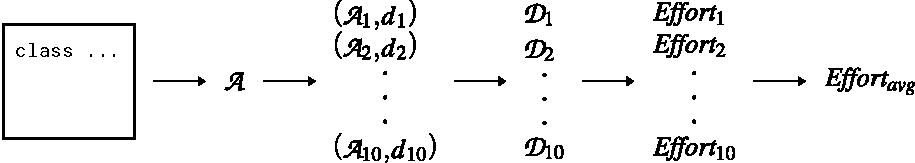
\includegraphics[width=\linewidth]{figures/fault_generation}
  \caption{An activity matrix $\mathcal{A}$ is generated for a particular class. Then, 10 fault candidates of cardinality 2 are generated with a corresponding activity matrix $\mathcal{A}_k$. For each generated matrix, we perform fault diagnosis with \emph{BARINEL} resulting in diagnostic report $\mathcal{D}_k$ and compute the wasted effort. Finally, we compute the average wasted effort. This process is repeated 10 times.}
  \label{fig:fault_generation}
\end{figure}

\begin{figure}
  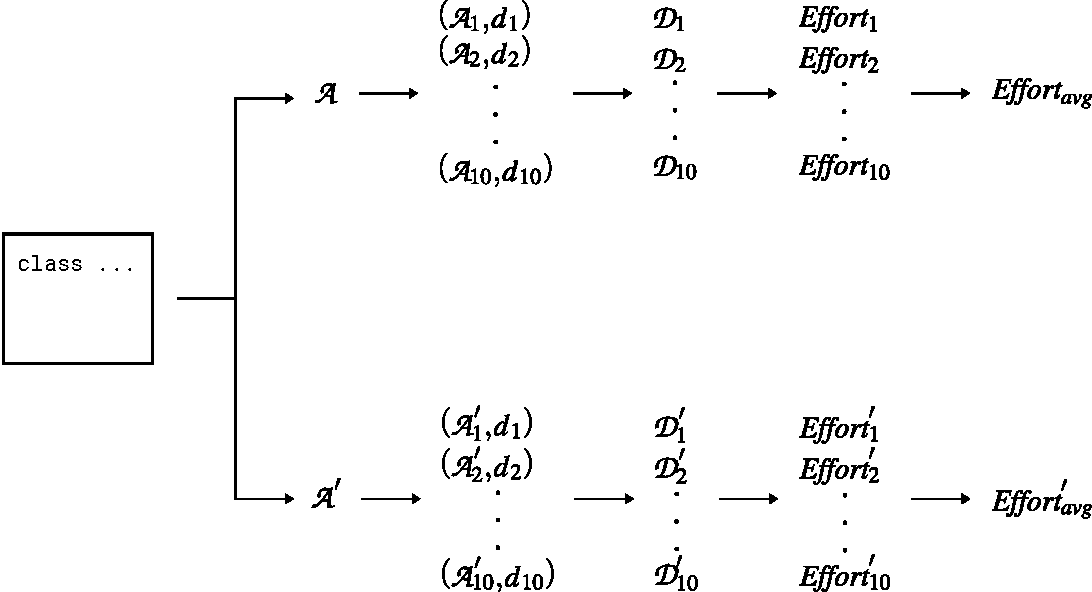
\includegraphics[width=\linewidth]{figures/fault_generation_delta}
  \caption{Two activity matrices $\mathcal{A}$ and $\mathcal{A}'$ are generated for a particular class based on two different test suites. We generate 10 fault candidates of cardinality 2 and accordingly generate 10 activity matrices. Then, we use \emph{BARINEL} to perform fault diagnosis and compute the wasted effort.}
  \label{fig:fault_generation_delta}
\end{figure}

In the construction of the activity matrix we use the branch granularity, that is, every component of the activity matrix represents a method branch; this granularity is also used by Perez \etal \cite{DBLP:conf/icse/PerezAD17}.
To construct the activity matrix of a class we use Perez' DDU Maven plugin\footnote{\url{https://github.com/aperez/ddu-maven-plugin}} using the \texttt{basicblock} granularity, which represents branch granularity.
The steps after the obtaining the activity matrix in \autoref{fig:fault_generation} are performed using Python scripts\footnote{\url{https://github.com/aaronang/ddu}}.

This experiment is different from Perez \etal's work because we do not improve the DDU of a fixed system.
Specifically, in Perez \etal's study, the authors improved the DDU of a fixed system under test by generating new test cases using \emph{EvoSuite}.
However, in this experiment, we compute the DDU for each class and measure for each class its diagnosability using the aforementioned approach.
Essentially, the difference is that we do not improve the DDU of a fixed system but we are simply measuring the DDU.



For this reason, we perform another experiment where we generate two test suites for each class with at least 8 components and at least 10 unit tests.
In addition, we perform the same experiment but for all classes with at least 8 components.
We generate two test suites by using all test cases and 50\% of the test cases.
For both test suites we compute the DDU and randomly generate 10 multiple components faults of cardinality 2 to compute the wasted effort.
Similar to previous experiment we perform this process 10 times to account for randomness of generating fault sets.
The intuition behind this experiment is when we improve the DDU of a fixed system, its diagnosability should improve too.
The setup of this experiment is illustrated in \autoref{fig:fault_generation_delta}.

\section{Experimental Results}
\label{sec:rq2_experimental_results}

\begin{figure*}
    \centering
    \begin{subfigure}[b]{0.49\linewidth}
        \centering
        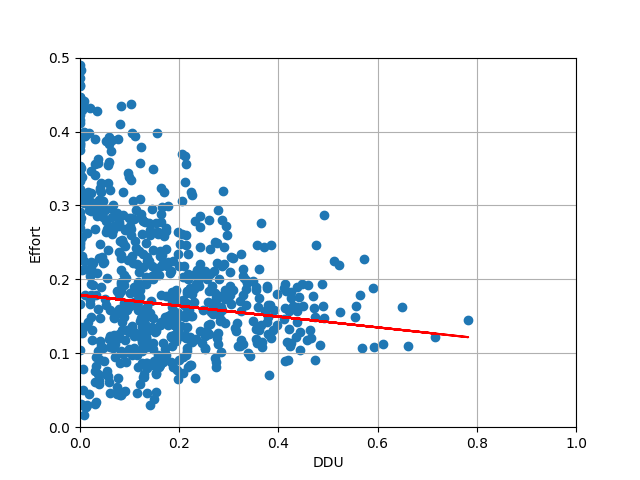
\includegraphics[width=\linewidth]{figures/ddu_effort_goodness_025}
        \caption{DDU, $r = -0.046$, $p = 0.224$.}
        \label{fig:ddu_effort_goodness_025}
    \end{subfigure}
    \hfill
    \begin{subfigure}[b]{0.49\linewidth}
        \centering
        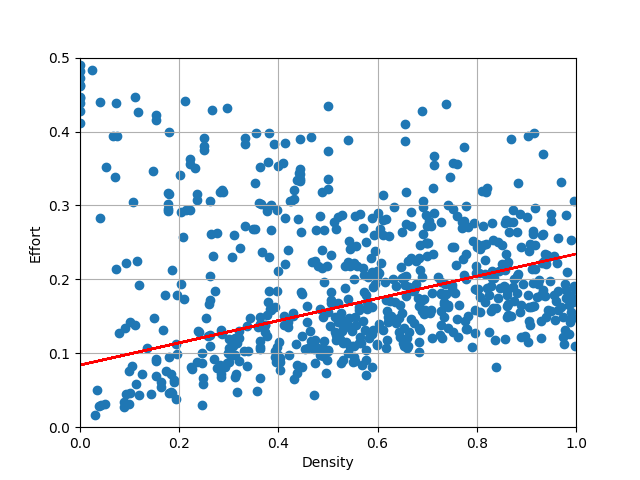
\includegraphics[width=\linewidth]{figures/density_effort_goodness_025}
        \caption{Density, $r = 0.183$, $p < 0.001$.}
        \label{fig:density_effort_goodness_025}
    \end{subfigure}
    \vskip\baselineskip
    \begin{subfigure}[b]{0.49\linewidth}
        \centering
        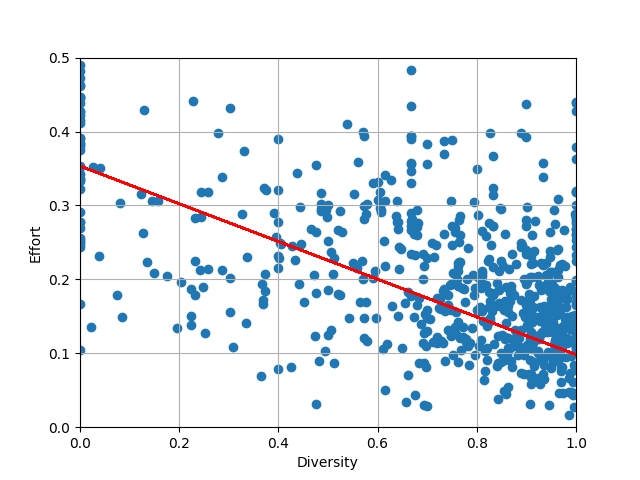
\includegraphics[width=\linewidth]{figures/diversity_effort_goodness_025}
        \caption{Diversity, $r = -0.326$, $p < 0.001$.}
        \label{fig:diversity_effort_goodness_025}
    \end{subfigure}
    \hfill
    \begin{subfigure}[b]{0.49\linewidth}
        \centering
        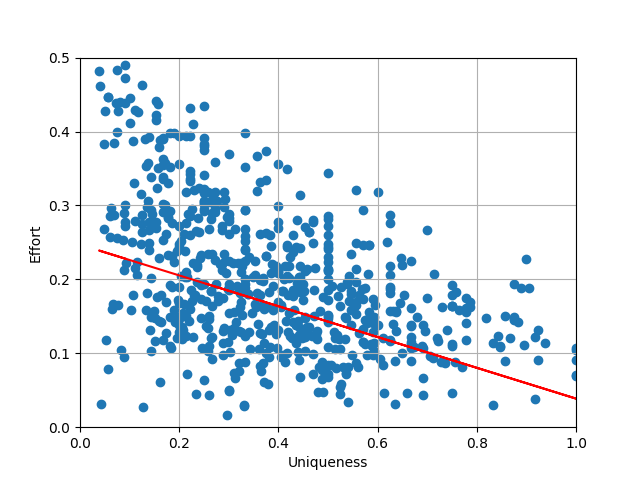
\includegraphics[width=\linewidth]{figures/uniqueness_effort_goodness_025}
        \caption{Uniqueness, $r = -0.120$, $p < 0.001$.}
        \label{fig:uniqueness_effort_goodness_025}
    \end{subfigure}
    \caption{Scatterplot of density, diversity, uniqueness, and DDU against effort.}
    \label{fig:metric_vs_effort}
\end{figure*}

In the first experiment, we measure for each class the density, diversity, uniqueness, DDU, and diagnosability.
The results of this experiment are shown in \autoref{fig:metric_vs_effort}.
Note that in \autoref{fig:metric_vs_effort} the population comprises all classes of all projects.
Each datapoint in \autoref{fig:metric_vs_effort} represents a class for which 100 fault candidates are generated in (potentially overlapping) sets of 10 fault candidates as described in \autoref{fig:fault_generation}.
We observe the that there is a positive correlation between density and effort, a negative correlation between diversity and effort, a negative correlation between uniqueness and effort, and a statistically non-significant weak correlation between DDU and effort.

To investigate the relations between these metrics in more detail, we display the correlation values per project in \autoref{tab:correlation_effort}.
For three projects we can say with 95\% confidence that density is correlated with effort.
However, the Pearson correlation for Commons Compress is negative while the Pearson correlation values for Commons Math and Commons Codec are positive.
Hence, the results show no strong evidence that density is correlated with effort.
Regarding diversity and uniqueness, we observe in \autoref{tab:correlation_effort} that both metrics are negatively correlated to effort, and that the correlation values in 4 out of 5 projects are statistically significant.
Regarding DDU, for two projects the results show statistical significance that DDU is negatively correlated to effort.
However, for three projects there is no evidence that DDU is correlated to effort.
Therefore, there is no strong evidence that DDU is negatively correlated to effort.

\begin{table}[]
\centering
\caption{Correlation between density, diversity, uniqueness, DDU, and effort.}
\label{tab:correlation_effort}
\begin{adjustbox}{center}
\begin{tabular}{llllll}
\toprule
 &  & \multicolumn{4}{c}{Pearson correlation / Correlation p-value} \\ \cline{3-6}
\multirow{-2}{*}{Subject} & \multirow{-2}{*}{Size} & Density & Diversity & Uniqueness & DDU \\
\rowcolor{Gray}
\cellcolor{Gray} & \cellcolor{Gray} & 0.63 & -0.33 & -0.65 & -0.23 \\
\rowcolor{Gray}
\multirow{-2}{*}{\cellcolor{Gray}\begin{tabular}[c]{@{}l@{}}Commons\\ Codec\end{tabular}} & \multirow{-2}{*}{\cellcolor{Gray}34} & $\mathbf{5.880\times10^{-5}}$ & 0.057 & $\mathbf{3.713\times10^{-5}}$ & 0.197 \\
 &  & -0.22 & -0.45 & -0.40 & -0.37 \\
\multirow{-2}{*}{\begin{tabular}[c]{@{}l@{}}Commons\\ Compress\end{tabular}} & \multirow{-2}{*}{104} & $\mathbf{0.027}$ & $\mathbf{1.348\times10^{-6}}$ & $\mathbf{2.083\times10^{-5}}$ & $\mathbf{1.121\times10^{-4}}$ \\
\rowcolor{Gray}
\cellcolor{Gray} & \cellcolor{Gray} & 0.20 & -0.36 & -0.19 & -0.03 \\
\rowcolor{Gray}
\multirow{-2}{*}{\cellcolor{Gray}\begin{tabular}[c]{@{}l@{}}Commons\\ Math\end{tabular}} & \multirow{-2}{*}{\cellcolor{Gray}420} & $\mathbf{4.982\times10^{-5}}$ & $\mathbf{1.782\times10^{-14}}$ & $\mathbf{7.553\times10^{-5}}$ & 0.572 \\
 &  & 0.01 & -0.31 & -0.29 & -0.22 \\
\multirow{-2}{*}{Guice} & \multirow{-2}{*}{94} & 0.935 & $\mathbf{0.002}$ & $\mathbf{0.005}$ & $\mathbf{0.031}$ \\
\rowcolor{Gray}
\cellcolor{Gray} & \cellcolor{Gray} & 0.29 & -0.37 & 0.16 & 0.20 \\
\rowcolor{Gray}
\multirow{-2}{*}{\cellcolor{Gray}Jsoup} & \multirow{-2}{*}{\cellcolor{Gray}37} & 0.085 & $\mathbf{0.024}$ & 0.337 & 0.229\\
\bottomrule
\end{tabular}
\end{adjustbox}
\end{table}

In the second experiment, we generate two test suites for a given class: a test suite with 50\% of the test cases enabled, and a test suite with 100\% of the test cases enabled.
This naturally results in two test suites with two different DDU values.
For each class, we compare the effort of a test suite with a lower DDU value with a test suite with a higher DDU value.
Identical approach is used for density, diversity, and uniqueness.
Note that we exclude classes where the two test suites do not result in a metric difference.
The results of this experiment are shown in \autoref{fig:delta_effort}, and the median effort and statistical test results for each subject are shown in \autoref{tab:statistical_test_delta_density}, \autoref{tab:statistical_test_delta_diversity}, \autoref{tab:statistical_test_delta_uniqueness}, and \autoref{tab:statistical_test_delta_ddu}.
We observe that $\emph{Effort}(\emph{DDU}_{HIGH})$ is statistically different in two cases out of five.
Hence, there is no strong evidence that improving the DDU for a class' test suite will improve diagnosability.

Revisiting the second research question:
\begin{framed}
\noindent
\textbf{RQ2:} What is the relation between density, diversity, uniqueness, and DDU and diagnosability?
\end{framed}
\textbf{A:} In the first experiment, two out of the five projects show that DDU is negatively correlated with diagnosability.
In the second experiment, two out of the five projects show that improving the DDU value of a class' test suite will improve the diagnosability.
Therefore, based on these two experiments, there is no strong evidence that DDU is correlated to diagnosability.
There is also no strong evidence that density, diversity, and uniqueness are correlated to diagnosability.

\begin{figure}
  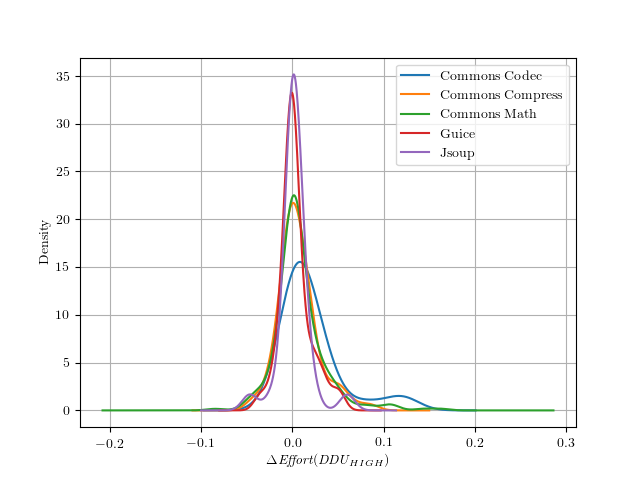
\includegraphics[width=\linewidth]{figures/delta_effort}
  \caption{}
  \label{fig:delta_effort}
\end{figure}

\begin{table}[]
\centering
\caption{Metrics and statistical tests related to density. Note that $t$ is computed using the t-test and $T$ is computed using the Wilcoxon signed-rank test.}
\label{tab:statistical_test_delta_density}
\begin{adjustbox}{center}
\begin{tabular}{llll}
\toprule
 &  & \multicolumn{2}{c}{Effort / Shapiro-Wilk / Statistical test} \\
\multirow{-2}{*}{Subject} & \multirow{-2}{*}{Size} & $\emph{Effort}(\emph{density}_{LOW})$ & $\emph{Effort}(\emph{density}_{HIGH})$ \\
\rowcolor{Gray}
\cellcolor{Gray} & \cellcolor{Gray} & 0.1617 & 0.1722 \\
\rowcolor{Gray}
\cellcolor{Gray} & \cellcolor{Gray} & $W = 0.9633$, $p\emph{-value} = 0.3968$ & $W = 0.9559$, $p\emph{-value} = 0.2609$ \\
\rowcolor{Gray}
\multirow{-3}{*}{\cellcolor{Gray}\begin{tabular}[c]{@{}l@{}}Commons\\ Codec\end{tabular}} & \multirow{-3}{*}{\cellcolor{Gray}29} & \multicolumn{2}{c}{\cellcolor{Gray}$t = 0.4314$, $p\emph{-value} = 0.6678$} \\
 &  & 0.1539 & 0.1539 \\
 &  & $W = 0.9587$, $p\emph{-value} = 0.0165$ & $W = 0.9582$, $p\emph{-value} = 0.0155$ \\
\multirow{-3}{*}{\begin{tabular}[c]{@{}l@{}}Commons\\ Compress\end{tabular}} & \multirow{-3}{*}{74} & \multicolumn{2}{c}{$T = 1340.0$, $p\emph{-value} = 0.9539$} \\
\rowcolor{Gray}
\cellcolor{Gray} & \cellcolor{Gray} & 0.1765 & 0.1720 \\
\rowcolor{Gray}
\cellcolor{Gray} & \cellcolor{Gray} & $W = 0.9696$, $p\emph{-value} = 3.5022\times10^{-5}$ & $W = 0.9682$, $p\emph{-value} = 2.2473\times10^{-5}$ \\
\rowcolor{Gray}
\multirow{-3}{*}{\cellcolor{Gray}\begin{tabular}[c]{@{}l@{}}Commons\\ Math\end{tabular}} & \multirow{-3}{*}{\cellcolor{Gray}251} & \multicolumn{2}{c}{\cellcolor{Gray}$T = 13967.0$, $p\emph{-value} = 0.2734$} \\
 &  & 0.1408 & 0.1464 \\
 &  & $W = 0.9711$, $p\emph{-value} = 0.0843$ & $W = 0.9749$, $p\emph{-value} = 0.1430$ \\
\multirow{-3}{*}{Guice} & \multirow{-3}{*}{75} & \multicolumn{2}{c}{$t = -0.0742$, $p\emph{-value} = 0.9408$} \\
\rowcolor{Gray}
\cellcolor{Gray} & \cellcolor{Gray} & 0.1078 & 0.1002 \\
\rowcolor{Gray}
\cellcolor{Gray} & \cellcolor{Gray} & $W = 0.9178$, $p\emph{-value} = 0.0268$ & $W = 0.9208$, $p\emph{-value} = 0.0320$ \\
\rowcolor{Gray}
\multirow{-3}{*}{\cellcolor{Gray}Jsoup} & \multirow{-3}{*}{\cellcolor{Gray}29} & \multicolumn{2}{c}{\cellcolor{Gray}$T = 176.0$, $p\emph{-value} = 0.3695$}\\
\bottomrule
\end{tabular}
\end{adjustbox}
\end{table}

\begin{table}[]
\centering
\caption{Metrics and statistical tests related to diversity. Note that $t$ is computed using the t-test and $T$ is computed using the Wilcoxon signed-rank test.}
\label{tab:statistical_test_delta_diversity}
\begin{adjustbox}{center}
\begin{tabular}{llll}
\toprule
 &  & \multicolumn{2}{c}{Effort / Shapiro-Wilk / Statistical test} \\
\multirow{-2}{*}{Subject} & \multirow{-2}{*}{Size} & $\emph{Effort}(\emph{diversity}_{LOW})$ & $\emph{Effort}(\emph{diversity}_{HIGH})$ \\
\rowcolor{Gray}
\cellcolor{Gray} & \cellcolor{Gray} & 0.1791 & 0.1881 \\
\rowcolor{Gray}
\cellcolor{Gray} & \cellcolor{Gray} & $W = 0.9678$, $p\emph{-value} = 0.6154$ & $W = 0.9685$, $p\emph{-value} = 0.6318$ \\
\rowcolor{Gray}
\multirow{-3}{*}{\cellcolor{Gray}\begin{tabular}[c]{@{}l@{}}Commons\\ Codec\end{tabular}} & \multirow{-3}{*}{\cellcolor{Gray}24} & \multicolumn{2}{c}{\cellcolor{Gray}$t = -0.2070$, $p\emph{-value} = 0.8368$} \\
 &  & 0.1584 & 0.1584 \\
 &  & $W = 0.9546$, $p\emph{-value} = 0.0103$ & $W = 0.9597$, $p\emph{-value} = 0.0199$ \\
\multirow{-3}{*}{\begin{tabular}[c]{@{}l@{}}Commons\\ Compress\end{tabular}} & \multirow{-3}{*}{73} & \multicolumn{2}{c}{$T = 1040.0$, $p\emph{-value} = 0.1241$} \\
\rowcolor{Gray}
\cellcolor{Gray} & \cellcolor{Gray} & 0.1767 & 0.1724 \\
\rowcolor{Gray}
\cellcolor{Gray} & \cellcolor{Gray} & $W = 0.9693$, $p\emph{-value} = 2.6065\times10^{-5}$ & $W = 0.9646$, $p\emph{-value} = 5.9871\times10^{-6}$ \\
\rowcolor{Gray}
\multirow{-3}{*}{\cellcolor{Gray}\begin{tabular}[c]{@{}l@{}}Commons\\ Math\end{tabular}} & \multirow{-3}{*}{\cellcolor{Gray}256} & \multicolumn{2}{c}{\cellcolor{Gray}$T = 13463.0$, $p\emph{-value} = 0.0649$} \\
 &  & 0.1410 & 0.1464 \\
 &  & $W = 0.9712$, $p\emph{-value} = 0.0856$ & $W = 0.9753$, $p\emph{-value} = 0.1512$ \\
\multirow{-3}{*}{Guice} & \multirow{-3}{*}{75} & \multicolumn{2}{c}{$t = -0.0574$, $p\emph{-value} = 0.9542$} \\
\rowcolor{Gray}
\cellcolor{Gray} & \cellcolor{Gray} & 0.1128 & 0.0998 \\
\rowcolor{Gray}
\cellcolor{Gray} & \cellcolor{Gray} & $W = 0.9211$, $p\emph{-value} = 0.0326$ & $W = 0.9158$, $p\emph{-value} = 0.0239$ \\
\rowcolor{Gray}
\multirow{-3}{*}{\cellcolor{Gray}Jsoup} & \multirow{-3}{*}{\cellcolor{Gray}29} & \multicolumn{2}{c}{\cellcolor{Gray}$T = 192.0$, $p\emph{-value} = 0.5813$}\\
\bottomrule
\end{tabular}
\end{adjustbox}
\end{table}

\begin{table}[]
\centering
\caption{Metrics and statistical tests related to uniqueness. Note that $t$ is computed using the t-test and $T$ is computed using the Wilcoxon signed-rank test.}
\label{tab:statistical_test_delta_uniqueness}
\begin{adjustbox}{center}
\begin{tabular}{llll}
\toprule
 &  & \multicolumn{2}{c}{Effort / Shapiro-Wilk / Statistical test} \\
\multirow{-2}{*}{Subject} & \multirow{-2}{*}{Size} & $\emph{Effort}(\emph{uniqueness}_{LOW})$ & $\emph{Effort}(\emph{uniqueness}_{HIGH})$ \\
\rowcolor{Gray}
\cellcolor{Gray} & \cellcolor{Gray} & 0.1758 & 0.1622 \\
\rowcolor{Gray}
\cellcolor{Gray} & \cellcolor{Gray} & $W = 0.9676$, $p\emph{-value} = 0.5624$ & $W = 0.9654$, $p\emph{-value} = 0.5104$ \\
\rowcolor{Gray}
\multirow{-3}{*}{\cellcolor{Gray}\begin{tabular}[c]{@{}l@{}}Commons\\ Codec\end{tabular}} & \multirow{-3}{*}{\cellcolor{Gray}26} & \multicolumn{2}{c}{\cellcolor{Gray}$t = -0.9103$, $p\emph{-value} = 0.3669$} \\
 &  & 0.1463 & 0.1463 \\
 &  & $W = 0.9378$, $p\emph{-value} = 0.0069$ & $W = 0.9445$, $p\emph{-value} = 0.0132$ \\
\multirow{-3}{*}{\begin{tabular}[c]{@{}l@{}}Commons\\ Compress\end{tabular}} & \multirow{-3}{*}{55} & \multicolumn{2}{c}{$T = 481.0$, $p\emph{-value} = \mathbf{0.0154}$} \\
\rowcolor{Gray}
\cellcolor{Gray} & \cellcolor{Gray} & 0.1662 & 0.1564 \\
\rowcolor{Gray}
\cellcolor{Gray} & \cellcolor{Gray} & $W = 0.9621$, $p\emph{-value} = 6.2737\times10^{-5}$ & $W = 0.9636$, $p\emph{-value} = 9.1669\times10^{-5}$ \\
\rowcolor{Gray}
\multirow{-3}{*}{\cellcolor{Gray}\begin{tabular}[c]{@{}l@{}}Commons\\ Math\end{tabular}} & \multirow{-3}{*}{\cellcolor{Gray}187} & \multicolumn{2}{c}{\cellcolor{Gray}$T = 5077.0$, $p\emph{-value} = \mathbf{8.5858\times10^{-7}}$} \\
 &  & 0.1348 & 0.1406 \\
 &  & $W = 0.9559$, $p\emph{-value} = 0.0455$ & $W = 0.9607$, $p\emph{-value} = 0.0747$ \\
\multirow{-3}{*}{Guice} & \multirow{-3}{*}{54} & \multicolumn{2}{c}{$T = 459.0$, $p\emph{-value} = 0.0558$} \\
\rowcolor{Gray}
\cellcolor{Gray} & \cellcolor{Gray} & 0.0979 & 0.0998 \\
\rowcolor{Gray}
\cellcolor{Gray} & \cellcolor{Gray} & $W = 0.8962$, $p\emph{-value} = 0.0110$ & $W = 0.9337$, $p\emph{-value} = 0.0853$ \\
\rowcolor{Gray}
\multirow{-3}{*}{\cellcolor{Gray}Jsoup} & \multirow{-3}{*}{\cellcolor{Gray}27} & \multicolumn{2}{c}{\cellcolor{Gray}$T = 83.0$, $p\emph{-value} = \mathbf{0.0108}$}\\
\bottomrule
\end{tabular}
\end{adjustbox}
\end{table}

\begin{table}[]
\centering
\caption{Metrics and statistical tests related to DDU. Note that $t$ is computed using the t-test and $T$ is computed using the Wilcoxon signed-rank test.}
\label{tab:statistical_test_delta_ddu}
\begin{adjustbox}{center}
\begin{tabular}{llll}
\toprule
 &  & \multicolumn{2}{c}{Effort / Shapiro-Wilk / Statistical test} \\
\multirow{-2}{*}{Subject} & \multirow{-2}{*}{Size} & $\emph{Effort}(\emph{DDU}_{LOW})$ & $\emph{Effort}(\emph{DDU}_{HIGH})$ \\
\rowcolor{Gray}
\cellcolor{Gray} & \cellcolor{Gray} & 0.1722 & 0.1454 \\
\rowcolor{Gray}
\cellcolor{Gray} & \cellcolor{Gray} & $W = 0.9593$, $p\emph{-value} = 0.3174$ & $W = 0.9655$, $p\emph{-value} = 0.4472$ \\
\rowcolor{Gray}
\multirow{-3}{*}{\cellcolor{Gray}\begin{tabular}[c]{@{}l@{}}Commons\\ Codec\end{tabular}} & \multirow{-3}{*}{\cellcolor{Gray}29} & \multicolumn{2}{c}{\cellcolor{Gray}$t = -0.8282$, $p\emph{-value} = 0.4110$} \\
 &  & 0.1583 & 0.1583 \\
 &  & $W = 0.9568$, $p\emph{-value} = 0.0129$ & $W = 0.9617$, $p\emph{-value} = 0.0247$ \\
\multirow{-3}{*}{\begin{tabular}[c]{@{}l@{}}Commons\\ Compress\end{tabular}} & \multirow{-3}{*}{74} & \multicolumn{2}{c}{$T = 974.0$, $p\emph{-value} = \mathbf{0.0384}$} \\
\rowcolor{Gray}
\cellcolor{Gray} & \cellcolor{Gray} & 0.1742 & 0.1717 \\
\rowcolor{Gray}
\cellcolor{Gray} & \cellcolor{Gray} & $W = 0.9699$, $p\emph{-value} = 2.5558\times10^{-5}$ & $W = 0.9619$, $p\emph{-value} = 2.1199\times10^{-6}$ \\
\rowcolor{Gray}
\multirow{-3}{*}{\cellcolor{Gray}\begin{tabular}[c]{@{}l@{}}Commons\\ Math\end{tabular}} & \multirow{-3}{*}{\cellcolor{Gray}262} & \multicolumn{2}{c}{\cellcolor{Gray}$T = 11308.0$, $p\emph{-value} = \mathbf{2.1258\times10^{-5}}$} \\
 &  & 0.1403 & 0.1464 \\
 &  & $W = 0.9722$, $p\emph{-value} = 0.0982$ & $W = 0.9744$, $p\emph{-value} = 0.1333$ \\
\multirow{-3}{*}{Guice} & \multirow{-3}{*}{75} & \multicolumn{2}{c}{$t = -0.3054$, $p\emph{-value} = 0.7604$} \\
\rowcolor{Gray}
\cellcolor{Gray} & \cellcolor{Gray} & 0.1078 & 0.1002 \\
\rowcolor{Gray}
\cellcolor{Gray} & \cellcolor{Gray} & $W = 0.9237$, $p\emph{-value} = 0.0379$ & $W = 0.9153$, $p\emph{-value} = 0.0233$ \\
\rowcolor{Gray}
\multirow{-3}{*}{\cellcolor{Gray}Jsoup} & \multirow{-3}{*}{\cellcolor{Gray}29} & \multicolumn{2}{c}{\cellcolor{Gray}$T = 155.0$, $p\emph{-value} = 0.1765$}\\
\bottomrule
\end{tabular}
\end{adjustbox}
\end{table}

\chapter{DDU vs. Error Detection}
\label{ch:rq2}
In this chapter, we discuss

\chapter{Conclusion}
\label{ch:conclusion}


\bibliographystyle{plain}
\bibliography{bibliography}

\end{document}
